\chapter{Simplicial Complexes and Homology}
\graphicspath{ {/home/tomasp/Dokumenty/Master_Thesis/figures/} }
%%Definitions, notations, remarks and examples
\theoremstyle{definition}
\newtheorem{definition}{Definition}[section]
\newtheorem{theorem}{Theorem}[section]
\newtheorem{lemma}{Lemma}[section]
\newtheorem{corollary}{Corollary}[section]
\newtheorem{example}{Example}[section]
\newtheorem*{remark}{Remark}

The goal of this and the following chapters is to establish and set up the pipeline for extracting the algebraic invariants of our data. Usually, we can only work with sampled and discrete data coming from some set of measurements. As such, we can't directly use methods of algebraic topology since we won't usually be working with discrete topological spaces and to properly use these methods, we would need an uncountable amount of data; something that isn't feasible from a computational point of view.
\par
This forces us to use different methods to somehow approximate and recover the topology of the ambient space given only a finite set of points. Secondly, we also need to consider the \textit{scale} of the data - some interesting properties may be more apparent only after we ``zoom'' in closely on them, some may not become apparent at all. All in all, we will construct the following pipeline:

\begin{center}
\smartdiagram[sequence diagram]{
  Discrete data, Simplicial complex, Algebraic invariants}
\end{center}

and repeat this step for all scales at once, effectively measuring the evolution of the algebraic invariants through the changes in the feature scale.

\section{Simplicial complexes}
\begin{definition}[Simplex]
For $k \geq 0$, a $k$-simplex $\sigma$ of dimension $k$ in an Euclidean space $\mathbb{R}^{n}$ is the convex hull of a set $P$ of $(k+1)$ affinely independent points in $\mathbb{R}^{n}$. For $0 \leq m \leq k$, an $m$-face of $\sigma$ is a $m$-simplex that is the convex hull of a nonempty subset of $P$. A \textit{proper face} of $\sigma$ is a simplex that is the convex hull of a proper subset of $P$ (any face except $\sigma$). $(k-1)$ faces of $\sigma$ are called \textit{facets} of $\sigma$.
\end{definition}

Typically we refer to a $0$-simplex as a \textit{vertex}, a $1$-simplex as an \textit{edge}, a $2$-simplex as a \textit{triangle} and so on. An illustration of those can be seen in \ref{fig:simplex_1}.

\begin{figure}[h!]
  \caption{From the left: a $0$-simplex, a $1$-simplex and a $2$-simplex}
  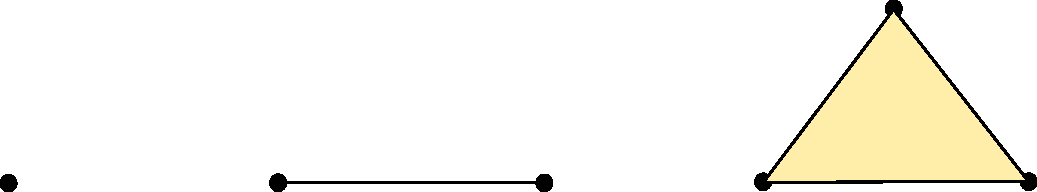
\includegraphics[width=10cm, height=2cm]{simplex_1.pdf}
  \centering
  \label{fig:simplex_1}
\end{figure}

\begin{definition}[Geometric simplicial complex]
  A \textit{geometric simplicial complex} $K$ is a set with finitely many simplices that satisfy the following:
  \begin{itemize}
    \item $K$ contains every face of each simplex in $K$.
    \item For any two simplices $\sigma, \tau \in K$, their intersection $\sigma \cap \tau$ is either empty or a face or both $\sigma$ and $\tau$.
  \end{itemize}
\end{definition}

This is also known as a \textit{triangulation}, where the \textit{dimension} $k$ of $K$ is the maximum dimension of any simplex in $K$. The two definitions above are highly geometric and easy to visualize and imagine. The next definition is more technical and abstract but nonetheless important.
